
\procTitle{Техносферные пожары: социально-экономические последствия
(на примере Магаданской области)}

\procAuthorI{Зеленцов~Н.\,С.}
\procEmailI{zelentsovnikita@mail.ru}
\procOrganizationI{ФГБУ СЭУ ФПС ИПЛ}
\procCityI{Магадан}

\procAuthorII{Лунегова~А.\,А., Болотин~А.\,В.}
\procEmailII{laaru@rambler.ru, alexandr\_bolotin@mail.ru}
\procOrganizationII{ФГБОУ ВО <<СВГУ>>}
\procCityII{Магадан}

\makeProcTitleII
\index{l@Лунегова~А.\,А.}
\index{b@Болотин~А.\,В.}
\index{z@Зеленцов~Н.\,С.}

Вопросы защищенности личности, имущества, общества и государства от пожаров являются приоритетными [4]. Возникновение пожаров и их последствия наносят огромный вред экономике страны. Пожары нарушают жизнь работников, работодателей и семей. В целях минимизации жертв и ущерба важно знать показатели возможной пожарной опасности объекта, её последствий для людей и имущества, то есть пожарный риск. Именно поэтому ситуация с пожарами требует дополнительного изучения, так как показатели по их количеству и последствиям заметно превышают количество и последствия происшествий иного характера.

Федеральным законом № 123-ФЗ установлено нормативное значение индивидуального пожарного риска (R$_H$), равное 10$^{-6}$ (1/чел.$\cdot$год) [3]. Для оценки пожарных рисков территорий (субъектов, городов, сельских поселений и др.) под руководством Н.~Н.~Брушлинского разработан ряд отдельных (частных) пожарных рисков [1], которые ориентированы на оценку социального и экономического ущерба (по отдельности друг от друга).

Социальные риски сопряжены с опасностью для людей. Для их оценки применены следующие показатели:
\begin{enumerate}[noitemsep]\vspace{-8pt}
  \item показатель R$_1$~--- подразумевает возможность человека столкнуться с пожаром при проживании или пользовании объектом и инфраструктурой:\\
  $$R_{1}=\frac{P}{N}\left(\dfrac{\text{пожар}}{\text{чел.}}\right),$$\\
  где Р~--- количество пожаров в год, ед.; N~--- количество людей, столкнувшихся с пожаром при проживании или пользовании объектом и~инфраструктурой, чел.;
  \item показатель R$_2$~--- подразумевает, что человек может пострадать при пожаре и сопутствующих обстоятельствах:\\
  $$R_{2}=\frac{N_\text{Ж}}{P}\left(\dfrac{\text{жертва}}{\text{пожаров}}\right),$$\\
  где N$_\text{Ж}$~--- количество жертв пожара, чел.; Р~--- количество пожаров в~год, ед.;
  \clearpage
  \item показатель R$_3$~--- характеризует опасность погибнуть при возгорании:\\
    $$R_{3}=\frac{N_\text{Ж}}{T}\left(\dfrac{\text{жертва}}{\text{год}}\right),$$\\
    где N$_\text{Ж}$~--- количество жертв пожара, чел.; T~--- промежуток времени, год.
\end{enumerate}
 \vspace{-8pt}

К экономическим рискам относятся риски, сопряжённые потерей материальных ценностей. Для их оценки применены показатели:
\begin{enumerate}[noitemsep]\vspace{-8pt}
  \item показатель R$_4$~--- характеризует риск уничтожения строений в результате пожара:\\
  $$R_{4}=\frac{N_\text{стр.}}{P}\left(\dfrac{\text{уничт. стр.}}{\text{пожар}}\right),$$\\
  где N$_\text{стр.}$~---  количество уничтоженных строений в результате пожара, ед.; Р~--- количество пожаров в~год, ед.;
  \item показатель R$_5$~--- характеризует риск прямого материального ущерба:\\
  $$R_{5}=\frac{D}{P}\left(\dfrac{\text{ден. ед.}}{\text{пожар}}\right),$$\\
    где D~--- сумма ущерба, руб.; Р~--- количество пожаров в~год, ед.
\end{enumerate}
 \vspace{-8pt}

 Разберём расчёт социальных и экономических последствий пожаров на~материалах Управления надзорной деятельности и профилактической работы Главного Управления МЧС России по Магаданской области [2]. На~рисунке 1 представлены данные о пожарах, жертвах и ущербе по Магаданской области.

\begin{figure}[H]
%\begin{changemargin}{-1cm}{0cm}
  \begin{center}
    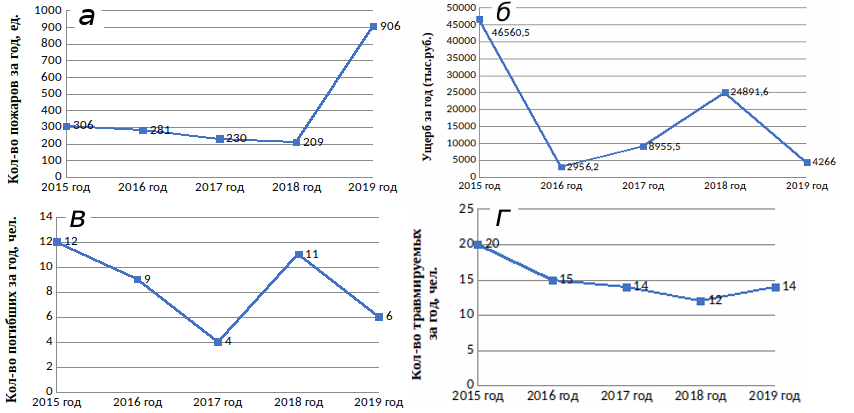
\includegraphics[width=1\textwidth]{authors/zelencov_fig1.png}
  \end{center}
%  \end{changemargin}
  \caption{Количество пожаров (\textit{а}); ущерб, причиненный пожарами (\textit{б}); количество погибших (\textit{в}) и~травмированных (\textit{г}) за 2015--2019 гг.}
  \label{fig:zelencov-fig1}
\end{figure}


Исходя из диаграммы рис. 1,\textit{а}, можно сделать вывод, что за 2019\,г., увеличился рост пожаров в Магаданской области (увеличение на 321,4\,\%) в~сравнении с аналогичными периодами.

Объектами возникновения пожаров были:
\begin{enumerate}[noitemsep]\vspace{-8pt}
  \item Жилой сектор~--- 210 пожаров (23,2\,\% от общего количества), увеличение на 42,9\,\%;
    \item Места открытого хранения веществ и материалов и прочие объекты~--- 578 пожаров (63,8\,\%), увеличение на 100\,\%;
      \item Транспортные средства~--- 47 пожаров (5,2\,\%), увеличение на 80,8\,\%;
        \item Здания учебно-воспитательного назначения~--- 1 пожар (0,1\,\%), увеличение на 100\,\%;
          \item Здания производственного назначения~--- 26 пожаров (2,9\,\%), увеличение на 85,7\,\%.
\end{enumerate}
 \vspace{-8pt}

 Исходя из диаграммы рис. 1,\textit{б}, мы видим, что прямой материальный ущерб причинен в размере 4266,4\,тыс. руб., снижение на 83,0\,\%, (20830,9\,тыс. руб. за 2018\,г.). Спасено материальных ценностей на сумму 29451,3\,тыс. руб.

 Исходя из диаграммы рис. 1,\textit{в}, можем наблюдать снижение количества погибших людей на 100\,тыс. населения на 45,5\,\% за 2019\,г. При пожарах погибло 6\,чел.

 Причины гибели людей на пожарах за 2019\,г.
\begin{enumerate}[noitemsep]\vspace{-8pt}
 \item Условия гибели: из 6 погибших при пожарах шестеро находились в~состоянии алкогольного опьянения;
 \item По социальному статусу среди погибших: 3 пенсионера, 1 рабочий, 2~БОРЗ;
 \item По возрастному показателю среди погибших: 1 чел. погиб в возрасте от 21 до 40 лет, 4 чел. погибло в возрасте от 41 до 60 лет, 1 чел. погиб в возрасте старше 60 лет.
\end{enumerate}
\vspace{-6pt}

Причинами возникновения пожаров с гибелью людей являются:
\begin{enumerate}[noitemsep]\vspace{-8pt}
\item Неосторожное обращение с огнем, (при курении)~--- 4 пожара (66,7\,\%), при которых погибло 4 чел. (66,7\,\%);
\item Неосторожность при приготовлении пищи 1 пожар (16,7\,\%), при котором погиб 1 чел. (16,7\,\%);
\item Нарушение правил эксплуатации электрооборудования 1 пожар (16,7\,\%), при котором погиб 1 чел. (16,7\,\%).
\end{enumerate}
\vspace{-6pt}

Исходя из диаграммы 1,\textit{г}, следует, что за 2019~г. при пожарах травмировано 14~чел. (увеличение на 16,7\,\% + 2~чел.).

Условия травмирования:
\begin{enumerate}[noitemsep]\vspace{-8pt}
\item Из 14 травмированных при пожаре 10~чел.  (71,4\,\%) находилось в состоянии алкогольного опьянения.
\item 14 чел. (100\,\%) проинструктированы по мерам пожарной безопасности.
\item По социальному статусу среди травмированных: 8~БОРЗ (53,8\,\%), 2~пенсионера (15,4\,\%), 3~рабочих (23,1\,\%), 1~индивидуальный предприниматель (7,7\,\%).
\item По возрастному показателю среди травмированных: 4~чел. (27,3\,\%) травмированы в возрасте от 21 до 40~лет, 8~чел. (63,7\,\%) травмированы в возрасте от 40 до 60~лет, 1~чел. (9,1\,\%) в возрасте старше 60~лет.
\end{enumerate}
\vspace{-8pt}

Причинами возникновения пожаров с травматизмом людей являются: аварийный режим работы электрооборудования~--- 3~пожара (23,0\,\%), при которых травмировано 3~чел. (23,0\,\%), неосторожное обращение с огнем, в~т.~ч. при курении~--- 10~пожаров (69,2\,\%), при которых травмировано 10~чел. (69,2\,\%), 1~пожар (7,7\,\%) прочие причины, 1~чел. (7,7\,\%) травмирован.

В 2015 г. среди трудоспособного населения во время пожаров, получило травмы различной степени тяжести 20~чел., среди них (17~чел. в~г.~Магадане, 2~чел. в~Сусуманском городском округе, 1~чел. в~Тенькинском городском округе, 1~чел. в~Хасынском городском округе).

В 2016 г. среди трудоспособного населения во время пожаров, получило травмы различной степени тяжести 15 чел., среди них (12~чел. в~г.~Магадане, 1~чел. в~Ольском городском округе, 1~чел. в~Северо-Эвенском городском округе, 1~чел. в~Сусуманском городском округе).

В 2017 г. среди трудоспособного населения во время пожаров, получило травмы различной степени тяжести 14 чел., среди них (12~чел. в~г. Магадане, 1~чел. в~Ольском городском округе, 1~чел. в~Сусуманском городском округе).

В 2018 г. среди трудоспособного населения во время пожаров, получило травмы различной степени тяжести 12 чел., среди них (9~чел. в~г. Магадане, 1~чел. в~Сусуманском городском округе, 2~чел. в~Ягоднинском городском округе).

В 2019 г. среди трудоспособного населения во время пожаров, получило травмы различной степени тяжести 14 чел., среди них (13~чел. в~г. Магадане, 1~чел. в~Хасынском городском округе).

Принимая во внимание причины гибели людей, количество пожаров на объектах гражданского строительства, причины возникновения пожаров, можно вынести следующие рекомендации и предложения по профилактике пожаров:
\begin{enumerate}[noitemsep]\vspace{-8pt}
  \item Совершенствовать работу по информационному обеспечению и противопожарной пропаганде.
  \item Задействовать личный состав пожарных подразделений на проверку жилых домов, обратив особое внимание при обследованиях на состояние электропроводки, электропроводки и печного отопления.
  \item Провести профилактические мероприятия с одинокими пенсионерами и инвалидами, неблагополучными семьями.
  \item Организовать и проводить мероприятия по обеспечению пожарной безопасности при подготовке жилого фонда к пожароопасным сезонам.
  \item Активизировать проведение комплекса противопожарных мероприятий, направленных на стабилизацию обстановки с пожарами в жилом фонде Магаданской области.
  \item Информирование людей о соблюдении требований пожарной безопасности путем размещения требований пожарной безопасности на квитанциях об оплате жилищно-коммунальных услуг и квитанциях об оплате за услуги в детских дошкольных образовательных учреждениях.
\end{enumerate}
\vspace{-8pt}

\begin{thebibliography}{99}
\bibitem{}Пожарные риски / Н.~Н.~Брушлинский, О.~В.~Иванова, Е.~А.~Клепко, С.~В.~Соколов, С.~Ю.~Попков.~--- М.~: Академия МЧС России, 2016.~--- 66~с.
\bibitem{}Статистические данные ФГБУ СЭУ ФПС ИПЛ по Магаданской области и УНД и ПР ГУ МЧС России по Магаданской области за 2015--2019 года.
\bibitem{}Федеральный закон Российской Федерации от 22 июля 2008 г. № 123-ФЗ  <<Технический регламент о требованиях пожарной безопасности>>.
\bibitem{}Федеральный закон Российской Федерации от 21.12.1994 № 69-ФЗ (ред. от 27.12.2019) <<О пожарной безопасности>>.
\end{thebibliography}
